\documentclass[border=6pt]{standalone}
\usepackage{tikz}
\usepackage{mathptmx}
\usetikzlibrary{shapes.geometric}
\definecolor{navy}{RGB}{20,52,110}
\definecolor{accent}{RGB}{14,110,120}
\definecolor{orange}{RGB}{200,110,30}
\definecolor{leaf}{RGB}{76,140,74}
\definecolor{landfill}{RGB}{225,235,228}
\begin{document}
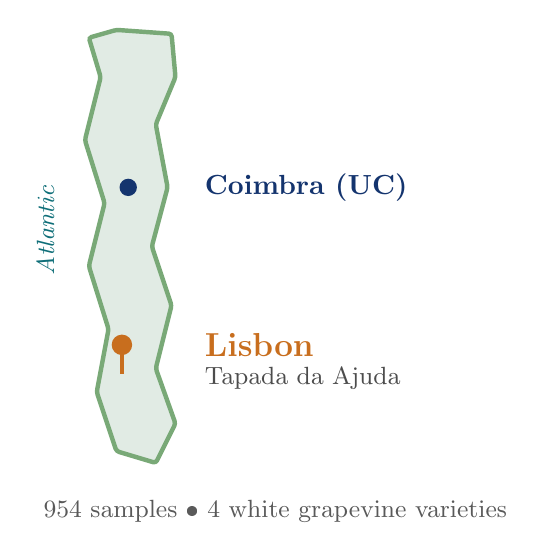
\begin{tikzpicture}[scale=1.0, font=\sffamily]
% --- stylised mainland Portugal outline (approximate) ---
\draw[line width=1.6pt, draw=leaf!75, fill=landfill, rounded corners=1pt]
  (0.55,5.55) -- (1.25,5.50) -- (1.30,4.95) -- (1.05,4.35) --
  (1.20,3.55) -- (1.00,2.80) -- (1.25,2.05) -- (1.05,1.25) --
  (1.30,0.55) -- (1.05,0.05) -- (0.55,0.20) -- (0.30,0.95) --
  (0.45,1.75) -- (0.20,2.55) -- (0.40,3.35) -- (0.15,4.15) --
  (0.35,4.95) -- (0.20,5.45) -- cycle;
% west coast hint (Atlantic label)
\node[font=\itshape\small, color=accent, rotate=90] at (-0.35,3.0) {Atlantic};
% --- Lisbon / Tapada da Ajuda pin (south-west) ---
\fill[orange] (0.62,1.55) circle (0.13);
\draw[line width=1.3pt, orange] (0.62,1.55) -- (0.62,1.18);
\node[anchor=west, font=\bfseries\large, color=orange] at (1.55,1.55) {Lisbon};
\node[anchor=west, font=\small, color=black!70] at (1.55,1.12) {Tapada da Ajuda};
% --- Coimbra pin (centre, where UC is) ---
\fill[navy] (0.70,3.55) circle (0.11);
\node[anchor=west, font=\bfseries, color=navy] at (1.55,3.55) {Coimbra (UC)};
% small caption
\node[font=\small, color=black!65, align=left, anchor=north west] at (-0.5,-0.3)
   {954 samples \textbullet\ 4 white grapevine varieties};
\end{tikzpicture}
\end{document}
